\documentclass{article}

% if you need to pass options to natbib, use, e.g.:
%     \PassOptionsToPackage{numbers, compress}{natbib}
% before loading neurips_2021

% ready for submission
% \usepackage{neurips_2021}

% to compile a preprint version, e.g., for submission to arXiv, add add the
% [preprint] option:
%     \usepackage[preprint]{neurips_2021}

% to compile a camera-ready version, add the [final] option, e.g.:
\usepackage[final]{neurips_2021}

% to avoid loading the natbib package, add option nonatbib:
%    \usepackage[nonatbib]{neurips_2021}

\usepackage[utf8]{inputenc} % allow utf-8 input
\usepackage[T1]{fontenc}    % use 8-bit T1 fonts
\usepackage{hyperref}       % hyperlinks
\usepackage{url}            % simple URL typesetting
\usepackage{booktabs}       % professional-quality tables
\usepackage{amsfonts}       % blackboard math symbols
\usepackage{nicefrac}       % compact symbols for 1/2, etc.
\usepackage{microtype}      % microtypography
\usepackage{xcolor}         % colors
\usepackage{graphicx}
\usepackage{float}

\title{ELEC 400m Reading Report}


\author{%
  Matthew C. Sam \\
  Department of Electrical and Computer Engineering\\
  University of British Columbia\\
  Vancouver, BC V6T 1Z4\\
  \texttt{mattsam@student.ubc.ca} \\
}

\begin{document}

\maketitle
\section{Introduction}

  Robotics is an inherently multidisciplinary field with many areas where machine learning techniques can be used. The goal of this paper will be to explore the applications of machine learning in legged robots. Applications such as applying deep reinforcement learning to teach a quadrupedal robot how to walk, and using inverse reinforcement learning to solve terrain traversability.

\section{Related Work}

One of the first questions that usually come up when it comes to legged robots is “why?”. Wheeled robots are simpler, faster, more stable, etc. Why should we make legged robots? My answer to this question is: We live in a world made for humans, designed by humans. Humans don’t have wheels. We need to traverse stairs and uneven terrain on a daily basis. Wheels simply are not fit for such tasks. If we want to build robots that can work in all the places that we can work but don’t want to radically change the way that we build our world then they should be able to move just like us.

\section{Methods/Applications}

\subsection{Deep Reinforcement Learning: Dreamer and DayDreamer}

Teaching robots to solve complex tasks in the real world is one of the main problems in robotics research. Deep reinforcement learning (DRL) is one of the tools often used when trying to have a robot learn a complex task. However, DRL has a few drawbacks in this application. It requires the robot to learn through trial and error which requires a large amount of interaction with its environment which is typically impractical for real-world usage. World models have shown promising results for learning how to play video games as well as learning in simulated domains. 

In the paper “DayDreamer: World Models for Physical Robot Learning” [1], The authors were able to have a quadrupedal robot learn how to get up and walk in an hour and deal with being pushed and knocked over in 10 min without using any simulations or demonstrations by leveraging the DRL and world-model learning. They used the Dreamer RL agent (developed by Google and Deepmind) [4] which had proven results on 20 difficult visual control tasks [2]. As shown in figure 1, their pipeline for using Dreamer followed four steps. The current learned policy collects experience. The experience is then added to the reply buffer. The world model is then trained on the replayed off-policy sequences through supervised learning. In the final step, the actor-critic algorithm optimizes a neural network policy from imagined rollouts in the latent space of the world model. They also parallelize the data collection and learning processes in order to learn while the robot is moving.

\begin{figure}[H]
  \centering
  \fbox{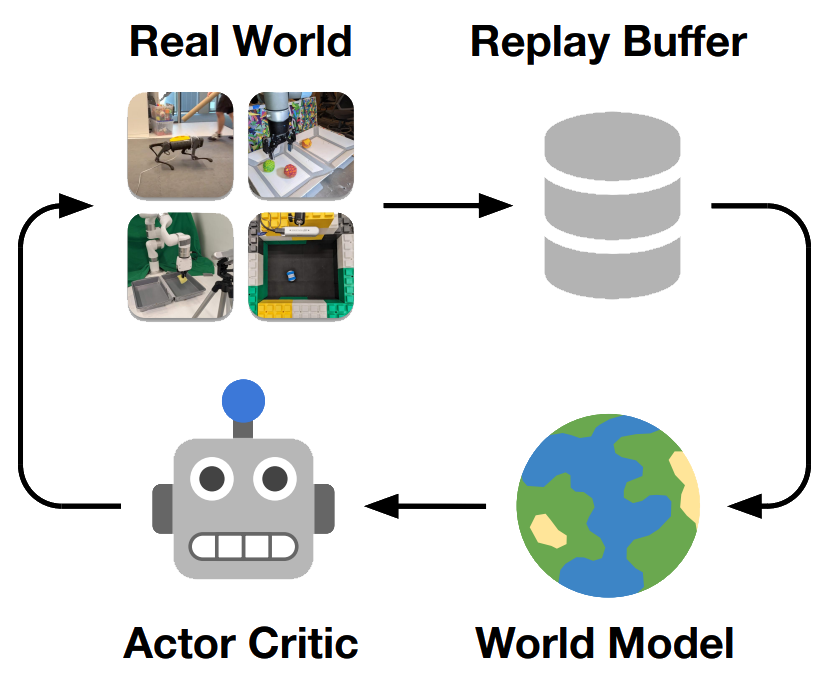
\includegraphics[width=5cm]{DREAM_algorithm.png}}%
  \caption{Illustration of DAYDREAMER pipeline [1]}
\end{figure}

Using this pipeline they were able to train a quadruped robot, seen in figure 2, to stand up and walk forward at a set velocity. Previous works that accomplished the same or similar tasks required large amounts of training in domain-randomized simulation with additional constraints such as recovery controllers to avoid unsafe states and having constraints in the joint trajectory generation. The authors of this paper were able to train in the end-to-end reinforcement learning setting without any of these additional constraints, although they did have to manually move the robot if it tried to move outside of their physical training area while maintaining any joint configurations and the orientation of the robot. 

\begin{figure}[H]
  \centering
  \fbox{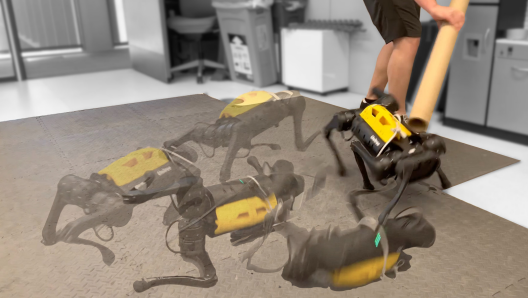
\includegraphics[width=5cm]{doog.png}}%
  \caption{Quadrupedal Robot Trained Using Dreamer [1]}
\end{figure}

\subsection{Energy-Based Transversability Using Deep Inverse Reinforcement Learning}

A large challenge for legged robots is autonomous navigation of unknown and unstructured environments. When using reinforcement learning to have a robot learn how to navigate unfamiliar terrain, demonstration of a human operator controlling the robot is often used as part of the reward structure. However, this approach leads to the trained robot rarely surpassing human control and the end reward function justifying the demonstrated behaviour rather than the underlying cause of the demonstrated behaviour. Energy consumption over a path is also a metric often used in evaluating a robot’s skill in traversing terrain, which is not something a human operator can easily be aware of when demonstrating the desired behaviour.

In their paper, Gan et al. [3] use deep inverse reinforcement learning (DIRL) to make a reward function that takes into account the average energy consumption over a path to create a more efficient policy than that which is created using demonstration. This reward network is trained using an extension of the maximum entropy deep reinforcement learning (MEDIRL) framework. These two functions are incorporated into a reward map. 

They detail their network structure as consisting of several branches as seen in figure 3. Whereas previous works use separate environmental and manually encoded kinematics in the reward function, in their paper Gan et al. instead allow the robot to learn its inertial features from its proprioceptive sensory data and integrating those results into the reward function. The proprioceptive data is processed using 1D convolutional modules. The inertial branch is designed in a similar way with 2 convolutional blocks, 1 fully connected layer, and a 1D max pooling layer. A dropout layer was also used as a model regularizer. The input of this branch is fixed-length data from the IMU. The third part of the network structure involved encapsulating the geometry and appearance of the local terrain into the reward learning. An elevation map was chosen and the ResUNet architecture for image segmentation was used as its base. These components were combined, as seen in figure 3, into a 2 stage architecture. In the first stage, the exteroceptive and proprioceptive data streams are processed individually and the environmental maps are generated. In the second stage, the results of the first step are fused using time stamps to create reward maps.

\begin{figure}[H]
  \centering
  \fbox{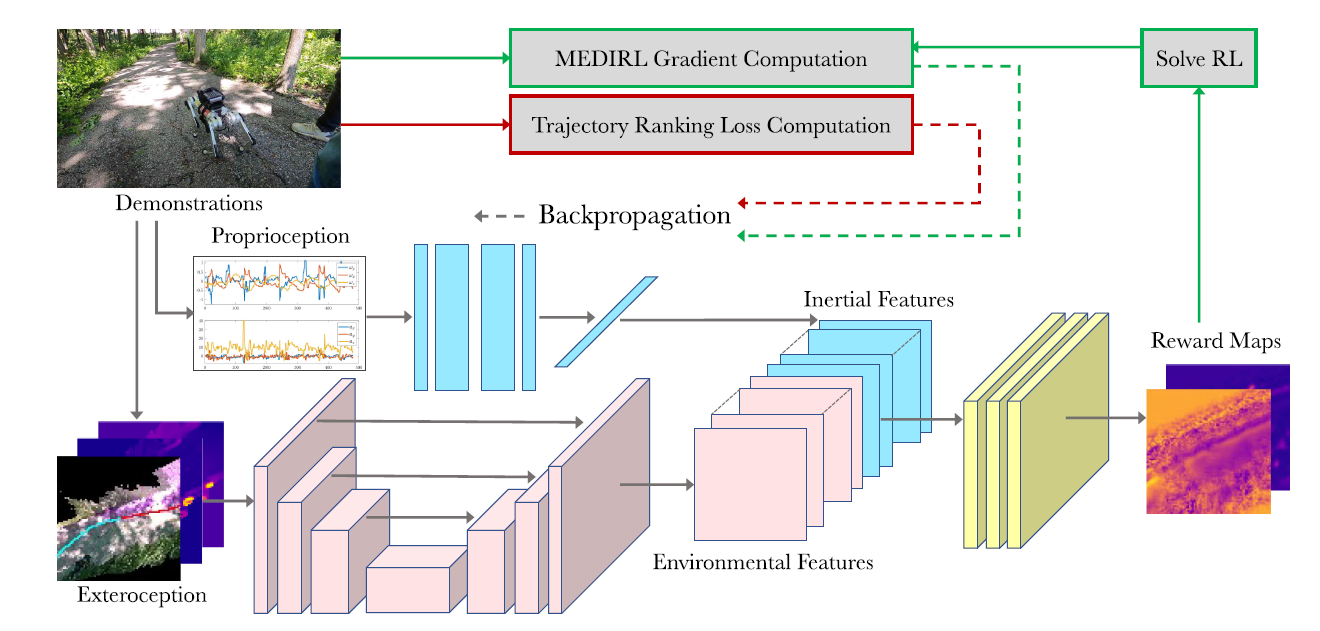
\includegraphics[width=13cm]{networkarch.png}}%
  \caption{Network Architecture [2]}
\end{figure}

The MEDIRL framework trains the reward network using stochastic gradient descent where the differences between the gradient from the demonstrated SVF and the expected SVF are evaluated. However, since the demonstration is known to be sub-optimal the MEDIRL framework needed to be augmented to allow for the extrapolation of rewards based on additional information. This was done by adding trajectory ranking loss to the existing framework. This new extension of the MEDIRL framework is T-MEDIRL. The “T” represents trajectories ranked by average energy consumption over their path. The idea of adding ranking loss was inspired by preference-based IRL which tries to learn the ranking over the demonstrations. The intention of this augmentation was to learn the intent rather than just the behaviour. 

The new methods were tested on a modified MIT Mini-cheetah robot with additional sensors. When compared to MEDIRL, T-MEDIRL had a worse NLL (higher loss) and HD (higher HD). However, T-MEDIRL performed better on the classification of higher reward trajectories as well as having a lower average energy consumption on the paths it chose.

\section{Discussion}
When I was searching for papers to use for my reading report my main goal was to see what the current state-of-the-art applications of machine learning in legged robotics are. After developing a shortlist of papers it became clear that reinforcement learning was one of the main machine learning techniques being used. Since reinforcement learning is not covered in this course I spent some time learning about it in order to try to connect the dots between what I know already and new concepts.

The DayDreamer paper involved teaching a quadrupedal robot to walk forwards as well as recover from being knocked over through the use of Dreamer. This paper was quite a challenging read and on top of deep RL, it also introduced the Dreamer framework as well as world-model learning. For me, this paper almost felt like an entirely different world from the machine learning I know right now. 

In contrast to the first paper, the paper on using deep inverse reinforcement learning to create energy-aware reward functions had a good mix of concepts that I have seen in this course, learned from other resources/courses, and those that are new to me. The section where the network architecture was explained was a good example of this. I found the idea of using machine learning to extrapolate the inaccuracies of human demonstration of the optimal way to perform a task particularly interesting.



\label{headings}

\section*{References}

{
\small

[1]P. Wu, A. Escontrela, D. Hafner, K. Goldberg, and P. Abbeel, “DayDreamer: World Models for Physical Robot Learning.” arXiv, 2022. doi: 10.48550/ARXIV.2206.14176.

[2]D. Hafner, T. Lillicrap, J. Ba, and M. Norouzi, “Dream to Control: Learning Behaviors by Latent Imagination.” arXiv, 2019. doi: 10.48550/ARXIV.1912.01603.

[3]L. Gan, J. W. Grizzle, R. M. Eustice, and M. Ghaffari, “Energy-based Legged Robots Terrain Traversability Modeling via Deep Inverse Reinforcement Learning,” arXiv, 2022, doi: 10.48550/ARXIV.2207.03034.


}

\end{document}